\documentclass[11pt]{article}
\usepackage{graphicx}
\usepackage{amssymb}
\usepackage{amsmath}
\usepackage{epstopdf}
\DeclareGraphicsRule{.tif}{png}{.png}{`convert #1 `dirname #1`/`basename #1 .tif`.png}

\textwidth = 6.5 in
\textheight = 9 in
\oddsidemargin = 0.0 in
\evensidemargin = 0.0 in
\topmargin = 0.0 in
\headheight = 0.0 in
\headsep = 0.0 in
\parskip = 0.2in
\parindent = 0.0in

\newtheorem{theorem}{Theorem}
\newtheorem{corollary}[theorem]{Corollary}
\newtheorem{definition}{Definition}

\newcommand{\cut}[1]{}

\title{The Matrix Calculus You Need For Deep Learning}
\author{Terence Parr and Jeremy Howard}
\begin{document}
\maketitle

\section{Introduction}

Most of us last saw calculus in school, but derivatives are a critical part of machine learning, particularly deep neural networks, which are trained by optimizing a loss function. Pick up a machine learning paper or the documentation of a library such as [PyTorch](link) and calculus comes screeching back into your life like distant relatives around the holidays.  And it's not just any old scalar calculus that pops up---we need differential {\em matrix calculus}, the shotgun wedding of [linear algebra](https://en.wikipedia.org/wiki/Linear\_algebra) and [multivariate calculus](https://en.wikipedia.org/wiki/Multivariable\_calculus).

For example, the activation of a single computation unit in a neural network is typically calculated using the dot product (from linear algebra) of an edge weight vector $\mathbf{w}$ with an input vector $\mathbf{x}$ plus a scalar bias (threshold): $z(\mathbf{x}) = \Sigma_i^n w_i x_i + b = \mathbf{w} \cdot \mathbf{x} + b$. Function $z(\mathbf{x})$ is called the unit's {\em affine function} and is followed by a [rectified linear unit](link), which clips negative values to zero: $max(0, z(\mathbf{x}))$. Such a computational unit is sometimes referred to as an ``artificial neuron'' and looks like:

\begin{center}
	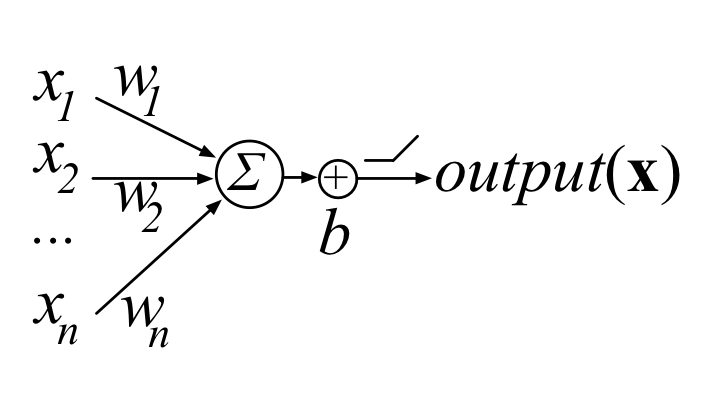
\includegraphics[scale=.9]{neuron.png}
\end{center}

Neural networks consist of many of these units, organized into multiple collections of neurons called {\em layers}. The activation of one layer's units become the input to the next layer's units. The activation of the unit or units in the final layer is called the network output.

{\em Training} this neuron means choosing weights $\mathbf{w}$ and bias $b$ so that we get the desired output for all inputs $\mathbf{x}$.  To do that, we minimize a {\em loss function} that compares the network's final $activation({\mathbf{x}})$ with the $target(\mathbf{x})$ (desired output of $\mathbf{x}$) for all input $\mathbf{x}$ vectors. To minimize the loss, we use some variation on gradient descent, such as plain [stochastic gradient descent](link) (SGD), SGD with momentum, [Adam](link).   All of those require the partial derivative (the gradient) of $activation({\mathbf{x}})$ with respect to the model parameters $\mathbf{w}$ and $b$. Our goal is to gradually tweak $\mathbf{w}$ and $b$ so that the overall loss function keeps getting smaller across all $\mathbf{x}$ inputs.

If we're careful, we can derive the gradient by differentiating the scalar version of a common loss function (mean squared error):

$\frac{1}{n} \Sigma_{\mathbf{x}} ||target(\mathbf{x}) - activation(\mathbf{x})||_2^2 = \frac{1}{n} \Sigma_{\mathbf{x}} ||target(\mathbf{x}) - max(0, \Sigma_i^n w_i x_i + b)||_2^2$

But this is just one neuron, and neural networks must train the weights and biases of all neurons in all layers simultaneously.  The really cool part about partial derivatives is that they let us optimize all of these network parameters at once. TODO: not sure "all at once" follows... Because there are multiple inputs and (potentially) multiple network outputs, we really need general rules for the derivative of a function with respect to a vector and even rules for the derivative of a vector-valued function with respect to a vector.

This article walks through the derivation of some important rules for computing partial derivatives with respect to vectors, particularly those useful for training neural networks. This field is known as {\em matrix calculus}, and the good news is, we only need a small subset of that field, which we introduce here.  While there is a lot of online material on multivariate calculus and linear algebra, they are typically taught as to separate undergraduate courses so most material treats them in isolation.  The pages that do discuss matrix calculus often are really just lists of rules with minimal explanation or are just pieces of the story.  In contrast, we're going to rederive and rediscover some key matrix calculus rules in an effort to explain them. It turns out that matrix calculus is really not that hard! There aren't dozens of new rules to learn; just a couple of key concepts.  That said, our intended audience already has many of these pieces in place mentally; it's more of a core dump than a complete textbook. Our hope is that it will get you started quickly in the world of matrix calculus related to training neural networks.

\section{Review: Scalar derivative rules}

Hopefully you remember some of these main scalar derivative rules. If your memory is a bit fuzzy on this, have a look at [khan vid](https://www.khanacademy.org/math/multivariable-calculus/multivariable-derivatives/differentiating-vector-valued-functions/a/multivariable-chain-rule-simple-version).

$
\begin{array}{lccc}
Rule & f(x) & \text{\parbox[t][0mm][b]{43mm}{Scalar derivative notation with respect to $x$}} & \text{Example}\\
\\[\dimexpr-\normalbaselineskip+2pt]
\hline
\\[\dimexpr-\normalbaselineskip+5pt]
\vspace{1mm}
\text{Constant} & c & 0 &  \frac{d}{dx}99 = 0\\
\vspace{1mm}
\text{Multiplication by constant} &	cf	&c \frac{df}{dx} & \frac{d}{dx}3x = 3\\
\vspace{1mm}
\text{Power Rule}	& x^n	& nx^{n-1} & \frac{d}{dx}x^3 = 3x^2\\
\vspace{1mm}
\text{Sum Rule}	& f + g	& \frac{df}{dx} + \frac{dg}{dx} & \frac{d}{dx} (x^2 + 3x) = 2x + 3\\
\vspace{1mm}
\text{Difference Rule}	& f - g	& \frac{df}{dx} - \frac{dg}{dx} & \frac{d}{dx}(x^2 - 3x) = 2x - 3\\
\vspace{1mm}
\text{Product Rule}	& fg & f \frac{dg}{dx} + \frac{df}{dx} g & \frac{d}{dx}x^2x = x^2 + x2x = 3x^2\\
\vspace{1mm}
\text{Quotient Rule}	& \frac{f}{g} = fg^{-1} & f \frac{dg}{dx}^{-1} + \frac{df}{dx} g^{-1} & \frac{d}{dx}x^2 / 3x = x^2/3 + 2x / 3x\\
\text{Chain Rule}	 & f(g(x)) &   \frac{df(u)}{du}\frac{du}{dx}, \text{ let } u=g(x) & \frac{d}{dx} ln(x^2) = \frac{1}{x^2}2x = \frac{2}{x}\\
\end{array}
$

There are other rules for trigonometry, exponentials, etc., which you can find [Khan Academy differential calculus course](https://www.khanacademy.org/math/differential-calculus).

When a function has a single parameter, $f(x)$, you'll often see $f'$ and $f'(x)$ used as shorthands for $\frac{d}{dx}f(x)$. We recommend against this notation as it does not make clear the variable we're taking the derivative with respect to. 

You can think of $\frac{d}{dx}$ as an operator that maps a function of one parameter to another function.  That means that $\frac{d}{dx} f(x)$ maps $f(x)$ to its derivative with respect to $x$, which is the same thing as $\frac{df(x)}{dx}$. Also, if $y = f(x)$, then $\frac{dy}{dx} = \frac{df(x)}{dx} = \frac{d}{dx}f(x)$. Thinking of the derivative as an operator helps to simplify complicated derivatives because the operator is distributive and lets us pull out constants. For example, in the following equation, we can pull out the constant 9 and distribute the derivative operator across the elements within the parentheses.

$\frac{d}{dx} 9(x + x^2) = 9 \frac{d}{dx}(x + x^2) = 9 (\frac{d}{dx}x + \frac{d}{dx}x^2) = 9(1 + 2x) = 9 + 18x$

That procedure reduced the derivative of $9(x + x^2)$ to a bit of arithmetic and the derivatives of $x$ and $x^2$, which are much easier to solve than the original derivative.

\section{Introduction to vector calculus and partial derivatives}

Neural network layers are not single functions of a single parameter, $f(x)$. So, let's move on to functions of multiple parameters such as $f(x,y)$. For example, what is the derivative of $xy$? In other words, how does the product $xy$ change when we wiggle the variables? Well, it depends on whether we are changing $x$ or $y$.  We compute derivatives with respect to one variable (parameter) at a time, giving us two different {\em partial derivatives} for this two-parameter function (one for $x$ and one for $y$).  Instead of using operator $\frac{d}{dx}$, the partial derivative operator is  $\frac{\partial}{\partial x}$ (a stylized $d$ and not the Greek letter $\delta$). So, $\frac{\partial }{\partial x}xy$ and $\frac{\partial }{\partial y}xy$ are the partial derivatives of $xy$; often, these are just called the {\em partials}.  For functions of a single parameter, operator $\frac{\partial}{\partial x}$ is equivalent to $\frac{d}{dx}$ (for sufficiently smooth functions). However, it's better to use to $\frac{d}{dx}$ to make it clear you're referring to a scalar derivative.

The partial derivative with respect to $x$ is just the usual scalar derivative, simply treating any other variable in the equation as a constant.  Consider function $f(x,y) = 3x^2y$. The partial derivative with respect to $x$ is written $\frac{\partial}{\partial x} 3x^2y$. There are three constants from the perspective of $\frac{\partial}{\partial x}$: 3, 2, and $y$. Therefore, $\frac{\partial}{\partial x} 3yx^2 = 3y\frac{\partial}{\partial x} x^2 = 3y2x = 6yx$. The partial derivative with respect to $y$ treats $x$ like a constant: $\frac{\partial}{\partial y} 3x^2y = 3x^2\frac{\partial}{\partial y} y = 3x^2\frac{\partial y}{\partial y} = 3x^2 \times 1 = 3x^2$.  It's a good idea to derive these yourself before continuing otherwise the rest of the article won't make sense.  Here's the [khan Academy video on partials](https://www.khanacademy.org/math/multivariable-calculus/multivariable-derivatives/partial-derivative-and-gradient-articles/a/introduction-to-partial-derivatives) if you need help.

So, partial derivatives use the usual scalar derivative rules while holding all but a single variable, $x$, as constants for the purpose of computing the partial derivative with respect to $x$.

To make it clear we are doing vector calculus and not just multivariate calculus, let's consider what we do with the partial derivatives $\frac{\partial f(x,y)}{\partial x}$ and $\frac{\partial f(x,y)}{\partial y}$ (another way to say $\frac{\partial}{\partial x}f(x,y)$ and $\frac{\partial }{\partial y}f(x,y)$) that we computed for $f(x,y) = 3x^2y$.  Instead of having them just floating around and not organized in any way, let's organize them into a horizontal vector. We call this vector the {\em gradient} of $f(x,y)$ and write it as:

$\nabla f(x,y)  = [ \frac{\partial f(x,y)}{\partial x}, \frac{\partial f(x,y)}{\partial y}] = [6yx, 3x^2]$

So the gradient of $f(x,y)$ is simply a vector of its partials. Gradients are part of the vector calculus world, which deals with functions that map $n$ scalar parameters to a single scalar.  Now, let's get crazy and consider derivatives of multiple functions simultaneously.

\section{Matrix calculus}

When we move from derivatives of one function to derivatives of many functions, we move from the world of vector calculus to matrix calculus. Let's compute partial derivatives for two functions, both of which take two parameters.  We can keep the same $f(x,y) = 3x^2y$ from the last section, but let's also bring in $g(x,y) = 2x + y^8$.  The gradient for $g$ has two entries, a partial derivative for each parameter:

$\frac{\partial g(x,y)}{\partial x} = \frac{\partial 2x}{\partial x} + \frac{\partial y^8}{\partial x} = 2\frac{\partial x}{\partial x} + 0 = 2 \times 1 = 1$

and

$\frac{\partial g(x,y)}{\partial y} = \frac{\partial 2x}{\partial y} + \frac{\partial y^8}{\partial y} = 0 + 8y^7 = 8y^7$

giving us gradient $\nabla g(x,y) = [1, 8y^7]$.

Gradient vectors organize all of the partial derivatives for a specific scalar function. If we have two functions, we can also organize their gradients into a matrix by stacking the gradients. When we do so, we get the {\em Jacobian matrix} (or just the {\em Jacobian}) where the gradients are rows:

$J =
\begin{bmatrix}
	\nabla f(x,y)\\
	\nabla g(x,y)
\end{bmatrix} = \begin{bmatrix}
\frac{\partial f(x,y)}{\partial x} & \frac{\partial f(x,y)}{\partial y}\\
\frac{\partial g(x,y)}{\partial x} & \frac{\partial g(x,y)}{\partial y}\\
\end{bmatrix} = \begin{bmatrix}
	6yx & 3x^2\\
	1 & 8y^7
\end{bmatrix}
$

Welcome to matrix calculus!

{\bf Note that there are multiple ways to represent the Jacobian.} We are using the so-called [numerator layout](https://en.wikipedia.org/wiki/Matrix\_calculus\#Layout\_conventions) but many papers and software will use the {\em denominator layout}. This is just transpose of the numerator layout Jacobian (flip it around its diagonal):

$
\begin{bmatrix}
	6yx & 1\\
	3x^2 & 8y^7
\end{bmatrix}
$

\subsection{Generalization of the Jacobian}

So far, we've looked at a specific example of a Jacobian matrix. To define the Jacobian matrix more generally, let's combine multiple parameters into a single vector argument: $f(x,y,z) \Rightarrow f(\mathbf{x})$. (You will sometimes see notation $\vec{x}$  for vectors in the literature as well.) Lowercase letters in bold font such as $\mathbf{x}$ are vectors and those in italics font like $x$ are scalars. $x_i$ is the $i^{th}$ element of vector $\mathbf{x}$ and is in italics because a single vector element is a scalar. We also have to define an orientation for vector $\mathbf{x}$. We'll assume that all vectors are vertical by default of size $n \times 1$:

$\mathbf{x} = \begin{bmatrix}
           x_1\\
           x_2\\
           \vdots \\
           x_n\\
           \end{bmatrix}$

With multiple scalar-valued functions, we can combine them all into a vector just like we did with the parameters. Let $\mathbf{y} = \mathbf{f}(\mathbf{x})$ be a vector of $m$ scalar-valued functions that each take a vector $\mathbf{x}$ of length $n=|\mathbf{x}|$ where $|\mathbf{x}|$ is the cardinality (count) of elements in $\mathbf{x}$. Each $f_i$ function within $\mathbf{f}$ returns a scalar just as in the previous section:

$
\begin{array}{lcl}
y_1 & = & f_1(\mathbf{x})\\
y_2 & = & f_2(\mathbf{x})\\
 & \vdots & \\
y_m & = & f_m(\mathbf{x})\\
\end{array}
$

For instance, we'd represent $f(x,y) = 3x^2y$ and $g(x,y) = 2x + y^8$ from the last section as

$y_1 = f_1(\mathbf{x}) = 3x_1^2x_2$ ~~~~~~~~(substituting $x_1$ for $x$, $x_2$ for $y$)\\
$y_2 = f_2(\mathbf{x}) = 2x_1 + x_2^8$

It's very often the case that $m=n$ because we will have a scalar function result for each element of the $\mathbf{x}$ vector.  For example, consider the identity function $\mathbf{y} = \mathbf{f(x)} = \mathbf{x}$:

$
\begin{array}{lclcc}
y_1 & = & f_1(\mathbf{x})& = & x_1\\
y_2 & = & f_2(\mathbf{x})& = & x_2\\
 & \vdots & \\
y_n & = & f_n(\mathbf{x})& = & x_n\\
\end{array}
$

So we have $m=n$ functions and parameters, in this case. Generally speaking, though, the Jacobian matrix is the collection of all $m \times n$ possible partial derivatives, which is the stack of $m$ gradients with respect to $\mathbf{x}$:

$
\frac{\partial \mathbf{y}}{\partial \mathbf{x}} = \begin{bmatrix}
\nabla f_1(\mathbf{x}) \\
\nabla f_2(\mathbf{x})\\
\ldots\\
\nabla f_m(\mathbf{x})
\end{bmatrix} = \begin{bmatrix}
\frac{\partial}{\partial \mathbf{x}} f_1(\mathbf{x}) \\
\frac{\partial}{\partial \mathbf{x}} f_2(\mathbf{x})\\
\ldots\\
\frac{\partial}{\partial \mathbf{x}} f_m(\mathbf{x})
\end{bmatrix} = \begin{bmatrix}
\frac{\partial}{\partial {x_1}} f_1(\mathbf{x})~ \frac{\partial}{\partial {x_2}} f_1(\mathbf{x}) ~\ldots~ \frac{\partial}{\partial {x_n}} f_1(\mathbf{x}) \\
\frac{\partial}{\partial {x_1}} f_2(\mathbf{x})~ \frac{\partial}{\partial {x_2}} f_2(\mathbf{x}) ~\ldots~ \frac{\partial}{\partial {x_n}} f_2(\mathbf{x}) \\
\ldots\\
~\frac{\partial}{\partial {x_1}} f_m(\mathbf{x})~ \frac{\partial}{\partial {x_2}} f_m(\mathbf{x}) ~\ldots~ \frac{\partial}{\partial {x_n}} f_m(\mathbf{x}) \\
\end{bmatrix}
$

where each $\frac{\partial}{\partial \mathbf{x}} f_i(\mathbf{x})$ is a horizontal $n$-vector because the partial derivative is with respect to a vector, $\mathbf{x}$, whose length is $n = |\mathbf{x}|$.  The width of the Jacobian is $n$ if we're taking the partial derivative with respect to $\mathbf{x}$ because there are $n$ parameters we can wiggle, each potentially changing the function's value. Therefore, the Jacobian is always $m$ rows for $n$ equations.  It helps to think about the possible Jacobian shapes visually:

\begin{center}
\begin{tabular}{c|ccl}
  & \begin{tabular}[t]{c}
  scalar\\
  \framebox(25,25){$x$}\\
  \end{tabular} & \begin{tabular}{c}
  vector\\
  \framebox(25,60){$\mathbf{x}$}
  \end{tabular}\\
\hline
\\[\dimexpr-\normalbaselineskip+5pt]
\begin{tabular}[b]{c}
  scalar\\
  \framebox(25,25){$f$}\\
  \end{tabular} &\framebox(25,25){$\frac{\partial f}{\partial {x}}$} & \framebox(60,25){$\frac{\partial f}{\partial {\mathbf{x}}}$}&\\
\begin{tabular}[b]{c}
  vector\\
  \framebox(25,60){$\mathbf{f}$}\\
  \end{tabular} & \framebox(25,60){$\frac{\partial \mathbf{f}}{\partial {x}}$} & \framebox(60,60){$\frac{\partial \mathbf{f}}{\partial \mathbf{x}}$}\\
\end{tabular}
\end{center}

The Jacobian of the identity function $\mathbf{f(x)} = \mathbf{x}$, with $f_i(\mathbf{x}) = x_i$, has $n$ functions and each function has $n$ parameters held in a single vector $\mathbf{x}$. The Jacobian is, therefore, a square matrix since $m=n$:

$
\begin{array}{lll}
\frac{\partial \mathbf{y}}{\partial \mathbf{x}} = \begin{bmatrix}
\frac{\partial}{\partial {x}} f_1(\mathbf{x}) \\
\frac{\partial}{\partial {x}} f_2(\mathbf{x})\\
\ldots\\
\frac{\partial}{\partial {x}} f_m(\mathbf{x})
\end{bmatrix} &=& \begin{bmatrix}
\frac{\partial}{\partial {x_1}} f_1(\mathbf{x})~ \frac{\partial}{\partial {x_2}} f_1(\mathbf{x}) ~\ldots~ \frac{\partial}{\partial {x_n}} f_1(\mathbf{x}) \\
\frac{\partial}{\partial {x_1}} f_2(\mathbf{x})~ \frac{\partial}{\partial {x_2}} f_2(\mathbf{x}) ~\ldots~ \frac{\partial}{\partial {x_n}} f_2(\mathbf{x}) \\
\ldots\\
~\frac{\partial}{\partial {x_1}} f_m(\mathbf{x})~ \frac{\partial}{\partial {x_2}} f_m(\mathbf{x}) ~\ldots~ \frac{\partial}{\partial {x_n}} f_m(\mathbf{x}) \\
\end{bmatrix}\\\\
 & = & \begin{bmatrix}
\frac{\partial}{\partial {x_1}} x_1~ \frac{\partial}{\partial {x_2}} x_1 ~\ldots~ \frac{\partial}{\partial {x_n}} x_1 \\
\frac{\partial}{\partial {x_1}} x_2~ \frac{\partial}{\partial {x_2}} x_2 ~\ldots~ \frac{\partial}{\partial {x_n}} x_2 \\
\ldots\\
~\frac{\partial}{\partial {x_1}} x_n~ \frac{\partial}{\partial {x_2}} x_n ~\ldots~ \frac{\partial}{\partial {x_n}} x_n \\
\end{bmatrix}\\\\
& & (\text{and since } \frac{\partial}{\partial {x_j}} x_i = 0 \text{ for } j \neq i)\\\\
 & = & \begin{bmatrix}
\frac{\partial}{\partial {x_1}} x_1 & 0 & \ldots& 0 \\
0 & \frac{\partial}{\partial {x_2}} x_2 &\ldots & 0 \\
& & \ddots\\
0 & 0 &\ldots& \frac{\partial}{\partial {x_n}} x_n \\
\end{bmatrix}\\\\
 & = & \begin{bmatrix}
1 & 0 & \ldots& 0 \\
0 &1 &\ldots & 0 \\
& & \ddots\\
0 & 0 & &1 \\
\end{bmatrix}\\\\
& = & I ~~~~(I \text{ is the identity matrix with ones down the diagonal})\\
\end{array}
$

Make sure that you can derive each step above before moving on. If you get stuck, just consider each element of the matrix in isolation and apply the usual scalar derivative rules.   That is a generally useful trick: Reduce vector expressions down to a set of scalar expressions and then take all of the partials, combining the results appropriately into vectors and matrices at the end.
 
Also be careful to track whether a matrix is vertical, $\mathbf{x}$, or horizontal, $\mathbf{x}^T$ where $\mathbf{x}^T$ means $\mathbf{x}$ transpose. Also make sure you pay attention to whether something is a scalar-valued function, $y = \framebox(10,7){}\,$, or a vector of functions (or a vector-valued function), $\mathbf{y} = \framebox(10,7){}\,$.



\subsection{Derivatives of vector element-wise binary operators}

Element-wise binary operations on vectors, such as vector addition $\mathbf{w} + \mathbf{x}$, are important because we can express many common vector operations, such as the multiplication of a vector by a scalar, as element-wise binary operations.   Examples that often crop up in deep learning are $max(\mathbf{x},\mathbf{y})$ and $\mathbf{x} > \mathbf{y}$ (returns a vector of ones and zeros). We can generalize the element-wise binary operations with notation $\mathbf{y} = \mathbf{f(w)} \bigcirc \mathbf{g(x)}$ where $m=n=|y|=|w|=|x|$. The $\bigcirc$ symbol represents any element-wise operator (such as $+$) and not the $\circ$ function composition operator.  Here's what equation $\mathbf{y} = \mathbf{f(w)} \bigcirc \mathbf{g(x)}$ looks like when we zoom in to examine the scalar equations:

$\begin{bmatrix}
           y_1\\
           y_2\\
           \vdots \\
           y_n\\
           \end{bmatrix} = \begin{bmatrix}
           f_{1}(\mathbf{w}) \bigcirc g_{1}(\mathbf{x})\\
           f_{n}(\mathbf{w}) \bigcirc g_{2}(\mathbf{x})\\
           \vdots \\
           f_{n}(\mathbf{w}) \bigcirc g_{n}(\mathbf{x})\\
         \end{bmatrix}$

where we write $n$ not $m$ equations vertically to emphasize the fact that the result of element-wise operators give $m=n$ sized vector results.

Using the ideas from the last section, we can see that the general case for the Jacobian with respect to $\mathbf{w}$ is the square matrix:

$
\frac{\partial \mathbf{y}}{\partial \mathbf{w}}  = \begin{bmatrix}
\frac{\partial}{\partial w_1} ( f_{1}(\mathbf{w}) \bigcirc g_{1}(\mathbf{x}) ) & \frac{\partial}{\partial w_2} ( f_{1}(\mathbf{w}) \bigcirc g_{1}(\mathbf{x}) ) & \ldots & \frac{\partial}{\partial w_n} ( f_{1}(\mathbf{w}) \bigcirc g_{1}(\mathbf{x}) )\\\\
\frac{\partial}{\partial w_1} ( f_{2}(\mathbf{w}) \bigcirc g_{2}(\mathbf{x}) ) & \frac{\partial}{\partial w_2} ( f_{2}(\mathbf{w}) \bigcirc g_{2}(\mathbf{x}) ) & \ldots & \frac{\partial}{\partial w_n} ( f_{2}(\mathbf{w}) \bigcirc g_{2}(\mathbf{x}) )\\\\
& \ldots\\\\
\frac{\partial}{\partial w_1} ( f_{n}(\mathbf{w}) \bigcirc g_{n}(\mathbf{x}) ) & \frac{\partial}{\partial w_2} ( f_{n}(\mathbf{w}) \bigcirc g_{n}(\mathbf{x}) ) & \ldots & \frac{\partial}{\partial w_n} ( f_{n}(\mathbf{w}) \bigcirc g_{n}(\mathbf{x}) )\\
\end{bmatrix}
$

and the Jacobian with respect to $\mathbf{x}$ is:

$
\frac{\partial \mathbf{y}}{\partial \mathbf{x}}  = \begin{bmatrix}
\frac{\partial}{\partial x_1} ( f_{1}(\mathbf{w}) \bigcirc g_{1}(\mathbf{x}) ) & \frac{\partial}{\partial x_2} ( f_{1}(\mathbf{w}) \bigcirc g_{1}(\mathbf{x}) ) & \ldots & \frac{\partial}{\partial x_n} ( f_{1}(\mathbf{w}) \bigcirc g_{1}(\mathbf{x}) )\\\\
\frac{\partial}{\partial x_1} ( f_{2}(\mathbf{w}) \bigcirc g_{2}(\mathbf{x}) ) & \frac{\partial}{\partial x_2} ( f_{2}(\mathbf{w}) \bigcirc g_{2}(\mathbf{x}) ) & \ldots & \frac{\partial}{\partial x_n} ( f_{2}(\mathbf{w}) \bigcirc g_{2}(\mathbf{x}) )\\\\
& \ldots\\\\
\frac{\partial}{\partial x_1} ( f_{n}(\mathbf{w}) \bigcirc g_{n}(\mathbf{x}) ) & \frac{\partial}{\partial x_2} ( f_{n}(\mathbf{w}) \bigcirc g_{n}(\mathbf{x}) ) & \ldots & \frac{\partial}{\partial x_n} ( f_{n}(\mathbf{w}) \bigcirc g_{n}(\mathbf{x}) )\\
\end{bmatrix}
$

That's quite a furball, but fortunately the Jacobian is very often a diagonal matrix, a matrix that is zero everywhere but the diagonal. Because this greatly simplifies the Jacobian, let's examine in detail when the Jacobian reduces to a diagonal matrix for element-wise operations. 

In a diagonal Jacobian, all elements off the diagonal are zero, $\frac{\partial}{\partial w_j} ( f_i(\mathbf{w}) \bigcirc g_i(\mathbf{x}) ) = 0$ where $j \neq i$. (Notice that we are taking the partial derivative with respect to $w_j$ not $w_i$.) Under what conditions are those off-diagonal elements zero? Precisely when $f_i$ and $g_i$ are contants with respect to $w_j$, $\frac{\partial}{\partial w_j} f_i(\mathbf{w}) = \frac{\partial}{\partial w_j} g_i(\mathbf{x}) = 0$.  Regardless of the operator, if those partial derivatives go to zero, the operation goes to zero, $0 \bigcirc 0 = 0$ no matter what, and the partial derivative of a constant is zero.

Those partials go to zero when $f_i$ and $g_i$ are not functions of $w_j$. We know that element-wise operations imply that $f_i$ is purely a function of $w_i$ and $g_i$  is purely a function of $x_i$. For example, $\mathbf{w}+\mathbf{x}$ sums $w_i + x_i$. Consequently,  $f_i(\mathbf{w}) \bigcirc g_i(\mathbf{x})$ reduces to $f_i(w_i) \bigcirc g_i(x_i)$ and the goal becomes $\frac{\partial}{\partial w_j} f_i(w_i) = \frac{\partial}{\partial w_j} g_i(x_i) = 0$. $f_i(w_i)$ and $g_i(x_i)$ look like a constants to the partial differentiation operator with respect to $w_j$ when $j \neq i$ so the partials are zero off the diagonal. (Notation $f_i(w_i)$ is technically an abuse of our notation because $f_i$ and $g_i$ are functions of vectors not individual elements. We should really write something like $\hat f_{i}(w_i) = f_{i}(\mathbf{w})$, but that would muddy the equations further, and programmers are comfortable overloading functions, so we'll proceed with the notation anyway.)  

We'll take advantage of this simplification later and refer to the constraint that $f_i(\mathbf{w})$ and $g_i(\mathbf{x})$ access at most $w_i$ and $x_i$, respectively, as the {\em element-wise diagonal condition}.

Under this condition, the elements along the diagonal of the Jacobian are $\frac{\partial}{\partial w_i} ( f_i(w_i) \bigcirc g_i(x_i) )$:

$
\frac{\partial \mathbf{y}}{\partial \mathbf{w}}  = \begin{bmatrix}
\frac{\partial}{\partial w_1} ( f_{1}(w_1) \bigcirc g_{1}(x_1) )\\
& \frac{\partial}{\partial w_2} (f_{2}(w_2) \bigcirc g_{2}(x_2) ) & &\text{\huge0}\\
& & \ldots \\
\text{\huge0}& & & \frac{\partial}{\partial w_n} (f_{n}(w_n) \bigcirc g_{n}(x_n) )
\end{bmatrix}
$

(The large ``0''s are a shorthand indicating all of the off-diagonal are 0.)

More succinctly, we can write:

$\frac{\partial \mathbf{y}}{\partial \mathbf{w}} = diag \left( \frac{\partial}{\partial w_1}(f_{1}(w_1) \bigcirc g_{1}(x_1)),~ \frac{\partial}{\partial w_2}(f_{2}(w_2) \bigcirc g_{2}(x_2)),~ \ldots,~ \frac{\partial}{\partial w_n}(f_{n}(w_n) \bigcirc g_{n}(x_n)) \right)$

and

$\frac{\partial \mathbf{y}}{\partial \mathbf{x}} = diag \left( \frac{\partial}{\partial x_1}(f_{1}(w_1) \bigcirc g_{1}(x_1)),~ \frac{\partial}{\partial x_2}(f_{2}(w_2) \bigcirc g_{2}(x_2)),~ \ldots,~ \frac{\partial}{\partial x_n}(f_{n}(w_n) \bigcirc g_{n}(x_n)) \right)$

where $diag(\mathbf{x})$ constructs a matrix whose diagonal elements are taken from vector $\mathbf{x}$: $diag(\mathbf{x}) = \mathbf{x}^T I$. $I$ represents the square identity matrix of appropriate dimensions that is zero everywhere but the diagonal, which contains all ones.

Because we do lots of simple vector arithmetic, the general function $\mathbf{f(w)}$ in the binary element-wise operation is often just the vector $\mathbf{w}$.  Any time the general function is a vector, we know that $f_i(\mathbf{w})$ reduces to $f_i(w_i) = w_i$. For example, vector addition $\mathbf{w + x}$ fits our element-wise diagonal condition because $\mathbf{f(w)} + \mathbf{g(x)}$ has scalar equations $y_i = f_i(\mathbf{w}) + g_i(\mathbf{x})$ that reduce to just $y_i = f_i(w_i) + g_i(x_i) = w_i + x_i$ with partial derivatives:

$\frac{\partial}{\partial w_i} ( f_{i}(w_i) + g_{i}(x_i) ) = \frac{\partial}{\partial w_i}(w_i + x_i) = 1 + 0 = 1$\\
$\frac{\partial}{\partial x_i} ( f_{i}(w_i) + g_{i}(x_i) ) = \frac{\partial}{\partial x_i}(w_i + x_i) = 0 + 1 = 1$

That gives us $\frac{\partial (\mathbf{w+x})}{\partial \mathbf{w}} = \frac{\partial (\mathbf{w+x})}{\partial \mathbf{x}} = I$, the identity matrix, because every element along the diagonal is 1.

Given the simplicity of this special case, $f_i(\mathbf{w})$ reducing to $f_i(w_i)$, you should be able to derive the Jacobians for the common element-wise binary operations on vectors:

$
\begin{array}{lllll}
\text{Op} & \text{Partial with respect to } \mathbf{w} & \text{Partial with respect to }\mathbf{x}\\
\hline\\

+ & \frac{\partial (\mathbf{w+x})}{\partial \mathbf{w}} = diag(\ldots \frac{\partial (w_i + x_i)}{\partial w_i} \ldots) = diag(\vec{1}) = I & \frac{\partial (\mathbf{w+x})}{\partial \mathbf{x}} =  I\\\\

- & \frac{\partial (\mathbf{w-x})}{\partial \mathbf{w}}  =  diag(\ldots\frac{\partial (w_i - x_i)}{\partial w_i}\ldots) =  diag(\vec{1})  =  I & \frac{\partial (\mathbf{w-x})}{\partial \mathbf{x}}  =  diag(\ldots\frac{\partial (w_i - x_i)}{\partial x_i}\ldots)  =  diag(-\vec{1})  =  -I \\\\

\otimes & \frac{\partial (\mathbf{w \otimes x})}{\partial \mathbf{w}}  =  diag(\ldots\frac{\partial (w_i \times x_i)}{\partial w_i} \ldots)  =  diag(\mathbf{x}) & \frac{\partial (\mathbf{w \otimes x})}{\partial \mathbf{x}}  =  diag(\mathbf{w})\\\\

\oslash & \frac{\partial (\mathbf{w \oslash x})}{\partial \mathbf{w}}  =  diag(\ldots\frac{\partial (w_i / x_i)}{\partial w_i}\ldots)  =  diag(\ldots \frac{1}{x_i} \ldots) & \frac{\partial (\mathbf{w \oslash x})}{\partial \mathbf{x}}  =  diag(\ldots \frac{-w_i}{x_i^2} \ldots)\\

\end{array}
$

The $\otimes$ and $\oslash$ operators are element-wise multiplication and division; $\otimes$ is sometimes called the {\em Hadamard product}. There isn't a standard notation for element-wise multiplication and division so where using an approach consistent with our general binary operation notation.

\subsection{Derivatives involving scalar expansion}

When we multiply or add scalars to vectors, we're implicitly expanding the scalar to a vector and then performing an element-wise binary operation. For example, adding scalar $z$  to vector $\mathbf{x}$, $\mathbf{y} = \mathbf{x} + z$,
is really
$\mathbf{y} = \mathbf{f(x)} + \mathbf{g}(z)$ where $\mathbf{f(x)} = \mathbf{x}$ and $\mathbf{g}(z) = \vec{1} z$. Notation $\vec{1}$ represents a vector of ones of appropriate length.  $z$ is any scalar that doesn't depend on $\mathbf{x}$, which is useful because then $\frac{\partial z}{\partial x_i} = 0$ for any $x_i$ and that will simplify our partial derivative computations. (It's okay to think of variable $z$ as a constant for our discussion here.)  Similarly, multiplying by a scalar, $\mathbf{y} = \mathbf{x} z$, is really $\mathbf{y} = \mathbf{f(x)} \otimes \mathbf{g}(z) = \mathbf{x} \otimes \vec{1}z$ where $\otimes$ is the element-wise  multiplication (Hadamard product) of the two vectors.

The partial derivatives of vector-scalar addition and multiplication with, respect to vector $\mathbf{x}$, using our element-wise rule:

$\frac{\partial \mathbf{y}}{\partial \mathbf{x}} = diag \left( \ldots \frac{\partial}{\partial x_i} ( f_i(x_i) \bigcirc g_i(z) ) \ldots \right)$

This follows because functions $\mathbf{f(x)} = \mathbf{x}$ and $\mathbf{g}(z) = \vec{1} z$ clearly satisfy our element-wise diagonal condition for the Jacobian (that $f_i(\mathbf{x})$ refer at most to $x_i$ and $g_i(z)$ refers to the $i^{th}$ value of the $\vec{1}z$ vector where $z$ doesn't depend on $\mathbf{x}$). 

Using the usual rules for scalar partial derivatives, we arrive at the following diagonal elements of the Jacobian for vector-scalar addition:
 
$\frac{\partial}{\partial x_i} ( f_i(x_i) + g_i(z) ) = \frac{\partial (x_i + z)}{\partial x_i} = \frac{\partial x_i}{\partial x_i} + \frac{\partial z}{\partial x_i} = 1 + 0 = 1$

So, $\frac{\partial}{\partial \mathbf{x}} ( \mathbf{x} + z ) = diag(\vec{1}) = I$.

Computing the partial derivative with respect to the scalar parameter $z$, however, results in a vertical vector, not a diagonal matrix. The elements of the vector are:
 
$\frac{\partial}{\partial z} ( f_i(x_i) + g_i(z) ) = \frac{\partial (x_i + z)}{\partial z} = \frac{\partial x_i}{\partial z} + \frac{\partial z}{\partial z} = 0 + 1 = 1$

Therefore, $\frac{\partial}{\partial z} ( \mathbf{x} + z ) = \vec{1}$.

The diagonal elements of the Jacobian for vector-scalar multiplication involve the product rule for scalar derivatives:

$\frac{\partial}{\partial x_i} ( f_i(x_i) \otimes g_i(z) ) = x_i  \frac{\partial z}{\partial x_i} + z  \frac{\partial x_i}{\partial x_i} = 0 + z = z$

So, $\frac{\partial}{\partial \mathbf{x}} ( \mathbf{x} z ) = diag(\vec{1}  z) = I z$. 

The partial derivative with respect to a scalar parameter $z$ is a vertical vector whose elements are:

$\frac{\partial}{\partial z} ( f_i(x_i) \otimes g_i(z) ) = x_i \frac{\partial z}{\partial z} + z \frac{\partial x_i}{\partial z} = x_i + 0 = x_i$

This gives us $\frac{\partial}{\partial z} ( \mathbf{x} z ) = \mathbf{x}$.

\subsection{Vector sum reduction}

Summing up the elements of a vector is an important operation in deep learning, such as the network loss function, but we can also use it as a way to simplify computing the derivative of vector dot product and other operations that reduce vectors to scalars.

Let $y = sum( \mathbf{f}(\mathbf{x})) = \Sigma_{i=1}^n f_i(\mathbf{x})$.  Notice we were careful here to leave the parameter as a vector $\mathbf{x}$ because each function $f_i$ could use all values in the vector, not just $x_i$. The sum is over the {\bf results} of the function and not the parameter. The gradient ($1 \times n$ Jacobian) of vector summation is:

$
\begin{array}{lcl}
\frac{\partial y}{\partial \mathbf{x}} & = & \begin{bmatrix} \frac{\partial y}{\partial x_1}, \frac{\partial y}{\partial x_2}, \ldots, \frac{\partial y}{\partial x_n} \end{bmatrix}\\\\
 & = & \begin{bmatrix} \frac{\partial}{\partial x_1} \Sigma_i f_i(\mathbf{x}),~ \frac{\partial}{\partial x_2} \Sigma_i f_i(\mathbf{x}),~ \ldots,~ \frac{\partial}{\partial x_n} \Sigma_i  f_i(\mathbf{x}) \end{bmatrix} \\\\
 & = & \begin{bmatrix} \Sigma_i \frac{\partial f_i(\mathbf{x})}{\partial x_1},~ \Sigma_i \frac{\partial f_i(\mathbf{x})}{\partial x_2},~ \ldots,~ \Sigma_i \frac{\partial f_i(\mathbf{x})}{\partial x_n}  \end{bmatrix}~~~~~~~~~~~~~~~(\text{move derivative inside }\Sigma)\\\\
\end{array}
$

(The summation inside the gradient elements can be tricky so make sure to keep your notation consistent.)

Let's look at the gradient of the simple $y = sum(\mathbf{x})$. The function inside the summation is just $f_i(\mathbf{x}) = x_i$ and the gradient is then:

$\nabla y = \begin{bmatrix} \Sigma_i \frac{\partial f_i(\mathbf{x})}{\partial x_1},~ \Sigma_i \frac{\partial f_i(\mathbf{x})}{\partial x_2},~ \ldots,~ \Sigma_i \frac{\partial f_i(\mathbf{x})}{\partial x_n}  \end{bmatrix} = \begin{bmatrix} \Sigma_i \frac{\partial x_i}{\partial x_1},~ \Sigma_i \frac{\partial x_i}{\partial x_2},~ \ldots,~ \Sigma_i \frac{\partial x_i}{\partial x_n}  \end{bmatrix}$

Because $\frac{\partial}{\partial x_j} x_i = 0$ for $j \neq i$, we can simplify to:

$\nabla y = \begin{bmatrix} \frac{\partial x_1}{\partial x_1},~ \frac{\partial x_2}{\partial x_2},~ \ldots,~ \frac{\partial x_n}{\partial x_n}  \end{bmatrix} = \begin{bmatrix}1, 1, \ldots, 1\end{bmatrix} = \vec{1}^T$

Notice that the result is a horizontal vector full of 1s, not a vertical vector, and so the gradient is $\vec{1}^T$. (The $T$ exponent represents the transpose of the indicated vector. In this case, it flips a vertical vector of ones to a horizontal vector.) It's very important to keep the shape of all of your vectors and matrices in order otherwise it's impossible to compute the derivatives of complex functions.

As another example, let's sum the result of multiplying a vector by a constant scalar.  If $y = sum(\mathbf{x} z)$ then $f_i(\mathbf{x},z) = x_i z$. The gradient is:

$
\begin{array}{lcl}
\frac{\partial y}{\partial \mathbf{x}} & = & \begin{bmatrix} \Sigma_i \frac{\partial}{\partial x_1} x_i z,~ \Sigma_i \frac{\partial }{\partial x_2} x_i z,~ \ldots,~ \Sigma_i \frac{\partial}{\partial x_n} x_i z  \end{bmatrix}\\\\
 & = & \begin{bmatrix} \frac{\partial}{\partial x_1} x_1 z,~ \frac{\partial }{\partial x_2} x_2 z,~ \ldots,~ \frac{\partial}{\partial x_n} x_n z  \end{bmatrix}\\\\
 & = & \begin{bmatrix} z, z, \ldots, z \end{bmatrix}\\\\
\end{array}
$

The derivative with respect to scalar variable $z$ is $1 \times 1$:

$
\begin{array}{lcl}
\frac{\partial y}{\partial z} & = & \frac{\partial}{\partial z} \Sigma_{i=1}^n (x_i+z)\\\\
& = & \Sigma_i \frac{\partial}{\partial z} (x_i+z)\\\\
& = & \Sigma_i (0 + 1)\\\\
& = & n
\end{array}
$

\subsection{Single-variable chain rule}

%https://calculus.subwiki.org/wiki/Proof_of_product_rule_for_differentiation_using_chain_rule_for_partial_differentiation

We can't compute partial derivatives of very complicated functions using just the basic matrix calculus rules we've seen so far.  For example, we can't take the derivative of nested expressions like $sum(\mathbf{w}+\mathbf{x})$. We need to be able to combine our basic vector rules using what we can call the {\em vector chain rule}.   Unfortunately, there are a number of rules for differentiation that fall under the name ``chain rule'' so we have to be careful which chain rule we're talking about. Part of our goal here is to clearly define and name three different chain rules, indicating in which situation they are appropriate. To get warmed up, we'll start with what we'll call the {\em single-variable chain rule} in this section, where we want the derivative of a scalar function with respect to a scalar. In the next section, we'll move on to an important concept called the {\em total derivative} and use it to define what we'll pedantically call the {\em single-variable total-derivative chain rule}. Then, we'll be ready for the vector chain rule in its full glory as needed for neural networks.

The chain rule in general is a divide and conquer strategy (like Quicksort) that breaks complicated expressions into subexpressions whose derivatives are easier to compute.  Its power derives from the fact that we can process each simple subexpression in isolation yet still combine the  intermediate results to get the correct overall result.

The chain rule comes into play when we need the derivative of an expression composed of nested subexpressions. So the single-variable chain rule  applies when confronted with expressions like $\frac{d}{dx} sin(x^2)$.  The outermost expression takes the $sin$ of an intermediate result, a nested subexpression that squares $x$. The chain rule is generically defined in terms of nested functions written as $f(g(x))$. (You will also see the chain rule defined using function composition $(f \circ g)(x)$, which is the same thing.)  Some sources write the derivative using shorthand notation $f'(g(x))g'(x)$, but that hides the fact that we are performing a variable substitution: $u = g(x)$, which we'll see shortly. It's better to define the [single-variable chain rule](http://m.wolframalpha.com/input/?i=chain+rule) of $f(g(x))$ explicitly so we never take the derivative with respect to the wrong variable.

To deploy the single-variable chain rule, follow these steps:

\begin{enumerate}
	\item Replace subexpressions with intermediate variables for both binary and unary operators; e.g., $\times$ is binary, squaring an expression is unary because there is a single operand of the square operator.
	\item Compute derivatives of the intermediate variables.
	\item Combine all derivatives of intermediate variables by multiplying them together to get the overall result.
	\item Substitute intermediate variables back in if any are referenced.
\end{enumerate}

The third step puts the ``chain'' in ``chain rule'' because it chains together intermediate results.

Let's try our process on $y = f(g(x)) = sin(x^2)$:

\begin{enumerate}
	\item Replace. Let $u = x^2$ represent subexpression $x^2$ (shorthand for $u(x) = x^2$). This gives us:\\
	$u = x^2$ ~~~~~~~~~~~~~~~~~~~~~~~~~~~(relative to definition $f(g(x))$, $g(x) = x^2$)\\
	$y = sin(u)$ ~~~~~~~~~~~~~~~~~~~~~~($y = f(u) = sin(u)$)\\
The order of these subexpressions does not affect the answer, but we recommend working in the reverse order of operations dictated by the nesting (innermost to outermost). That way, expressions and derivatives are always functions of previously-computed elements. 
	\item Compute derivatives.\\
	$\frac{du}{dx} = 2x$ ~~~~~~~~~~~~~~~~~~~~~~~~~ (Take derivative with respect to $x$)\\
	$\frac{dy}{du} = cos(u)$  ~~~~~~~~~~~~~~~~~~~~ (Take derivative with respect to $u$ not $x$)
	\item Combine.\\
	$\frac{dy}{dx} = \frac{dy}{du} \frac{du}{dx} = cos(u)2x$
	\item Subtitute.\\
	$\frac{dy}{dx} = \frac{dy}{du} \frac{du}{dx} = cos(x^2)2x = 2xcos(x^2)$	
\end{enumerate}

Notice how easy it is to compute the derivatives of the intermediate variables in isolation! The chain rule says it's legal to do that and tells us how to combine the intermediate results to get $2xcos(x^2)$. 

You can think of the combining step of the chain rule in terms of units canceling. If we let $y$ be gallons of gas, $x$ be the gallons in a gas tank, and $u$ as miles we can interpret $\frac{dy}{dx} = \frac{dy}{du} \frac{du}{dx}$ as $\frac{miles}{tank} = \frac{miles}{gallon} \frac{gallon}{tank}$. The $gallon$ denominator and numerator cancel. This is a convenient way to remember the chain rule but the analogy only goes so far; don't treat $dy$ and $dx$ has separate variables since they are two components in the name of a single derivative operator.

Another way to to think about the single-variable chain rule is to visualize the overall expression as a dataflow diagram (or [abstract syntax tree](link) for compiler people):

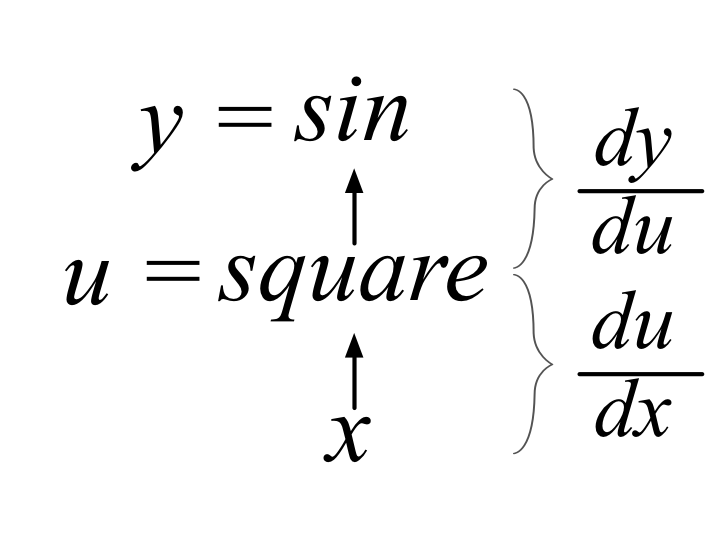
\includegraphics{sin-square.png}

Changes to function parameter $x$ bubble up through a squaring operation then through a $sin$ operation to change result $y$. You can think of $\frac{du}{dx}$ as ``getting changes from $x$ to $u$ and $\frac{dy}{du}$ as ``getting changes from $u$ to $y$.'' Getting from $x$ to $y$ requires an intermediate hop so we arrive at the single-variable chain rule. The chain rule is usually written from the output variable down to the parameters, $\frac{dy}{dx} = \frac{dy}{du} \frac{du}{dx}$. But, the $x$-to-$y$ perspective would be more clear if we used the equivalent $\frac{dy}{dx} = \frac{du}{dx}\frac{dy}{du}$.

\framebox[\linewidth]{\parbox{0.97\linewidth}{As an aside for those interested in automatic differentiation, papers and library documentation use terminology {\em forward differentiation} and {\em backward differentiation} (for use in the [back-propagation algorithm](link)). From a dataflow perspective, we are computing a forward differentiation because it follows the normal data flow direction.  Backward differentiation, naturally, goes the other direction and we're asking how a change in the output would affect function parameter $x$. Because backward differentiation can determine changes in all function parameters at once, it turns out to be much more efficient for functions with lots of parameters. Forward differentiation, on the other hand, must consider how a change in each parameter, in turn, affects the function output $y$.\\

\begin{tabular}{cc}
	Forward differentiation & Backward differentiation\\
	from $x$ to $y$ & from $y$ to $x$\\
$\frac{dy}{dx} = \frac{du}{dx}\frac{dy}{du}$ & $\frac{dy}{dx} = \frac{dy}{du} \frac{du}{dx}$\\
\end{tabular}
\vspace{3mm}

Automatic differentiation is beyond the scope of this article, but we're setting the stage for a future article.
}}

{\bf Conditions under which the single-variable chain rule applies}. Notice that there is a single dataflow path from $x$ to the root $y$. That is the condition under which we can apply the single-variable chain rule: when broken into individual binary and unary subexpressions, at most one subexpression can reference $x$. If there were references to $x$ in multiple subexpressions, even something simple like $x+x^2$, there'd be multiple paths from $x$ to the root.  To handle that situation, we'll learn about the single-variable total-derivative chain rule in the next section.
	
Many readers can solve $\frac{d}{dx}sin(x^2)$ in their heads, but our goal is a process that will work even for  very complicated expressions. This process is also how [automatic differentiation](link) works in libraries like PyTorch. So, by solving derivatives manually  in this way, you're also learning how to define functions for custom neural networks in PyTorch.

With deeply nested expressions, it helps to think about deploying the chain rule the way a compiler unravels function call nesting like $f_4(f_3(f_2(f_1(x))))$ into a sequence of calls. The result of calling function $f_i$ is saved to a temporary variable called a register, which is then passed as a parameter to $f_{i+1}$.  Let's see how that looks in practice by using our process on a highly-nested equation like $y = f(x) = ln(sin(x^3)^2)$:

\begin{enumerate}
	\item Replace.\\
$r_1 = f_1(x) = x^3$\\
$r_2 = f_2(r_1) = sin(r_1)$\\
$r_3 = f_3(r_2) = r_2^2$\\
$r_4 = f_4(r_3) = ln(r_3)$ ~~~~~~($y = r_4$)
	\item Compute derivatives.\\
$\begin{array}{lllll}
\vspace{1mm}
\frac{d}{r_x} r_1 & = & \frac{d}{x} x^3 & = & 3x^2\\
\vspace{1mm}
\frac{d}{r_1} r_2 & = & \frac{d}{r_1} sin(r_1) & = & cos(r_1) \\
\frac{d}{r_2} r_3 & = & \frac{d}{r_2} r_2^2 & =& 2r_2\\
\frac{d}{r_3} r_4 & = & \frac{d}{r_3} ln(r_3) & =& \frac{1}{r_3}\\
\end{array}$
	\item Combine four intermediate values.\\
$\frac{dy}{dx} = \frac{d r_4}{dx} = \frac{d r_4}{dr_3}\frac{dr_3}{d r_2} \frac{dr_2}{dr_1} \frac{dr_1}{dx} = \frac{1}{r_3}  2r_2  cos(r_1)  3x^2 = \frac{6r_2x^2cos(r_1)}{r_3}$
	\item Subtitute.\\
$\frac{dy}{dx} = \frac{6sin(r_1)x^2cos(x^3)}{r_2^2} = \frac{6sin(x^3)x^2cos(x^3)}{sin(r_1)^2} = \frac{6sin(x^3)x^2cos(x^3)}{sin(x^3)^2} = \frac{6x^2cos(x^3)}{sin(x^3)}$
\end{enumerate}


Here is a visualization of the data flow through the chain of operations from $x$ to $y$:

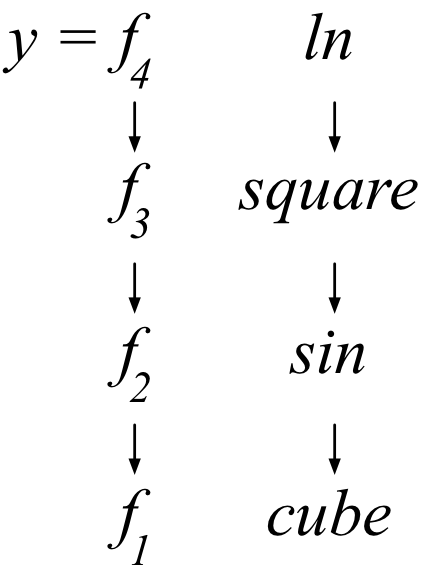
\includegraphics{chain-tree.png}

At this point, we can handle derivatives of nested expressions of a single variable, $x$. Moreover, we can only handle expressions that reference $x$ once and so we need to extend our technique, which we'll do in the next section.
 
\subsection{Vector chain rule}

Previously, we manually computed the derivative with respect to $\mathbf{x}$ of $y = sum(\mathbf{x}  z)$ as $[z, z, \ldots, z]$, but we can also use the chain rule. Let vector $\mathbf{u} = \mathbf{x}  z$ then $y = sum(\mathbf{u})$. The vector chain rule works just like the single-variable chain rule except that our variable is now a vector.  The vector general says that $\frac{dy}{d\mathbf{x}} = \frac{dy}{d\mathbf{u}}  \frac{d\mathbf{u}}{d\mathbf{x}}$, which means 

$\frac{dy}{d\mathbf{x}} = \vec{1}^T  \frac{d}{d\mathbf{x}} (\mathbf{x}  z) = \vec{1}^T  diag(\vec{1}z) = \vec{1}^T  I  z = \vec{1}^T  z = [z, z, \ldots, z]$

\pagebreak
{\bf NOTES}

Need [law of total derivative](https://en.wikipedia.org/wiki/Total\_derivative)

position $y = distance/time * time$ bump $delta y = distance/time * delta time$

{\bf Ex.} Let $f(x,y) = sin(xy)$. Substitute $u = xy$, giving $f(x,y) = sin(u(x,y))$ or just $sin(u)$. Chain rule says

$\frac{\partial f}{\partial x} = \frac{\partial f}{\partial u}\frac{\partial u}{\partial x} = cos(u)y = cos(xy)y$

and

$\frac{\partial f}{\partial y} = \frac{\partial f}{\partial u}\frac{\partial u}{\partial y} = cos(u)x = cos(xy)x$

General chain rule says $\frac{\partial}{\partial t} f(x(t),y(t)) = \frac{\partial f}{\partial x}\frac{\partial x}{\partial t} + \frac{\partial f}{\partial y}\frac{\partial y}{\partial t}$. Where is $t$ in my $sin(xy)$??? AND, where is the addition it says I need? How do I get partial w.r.t. $x$ or $y$?

{\bf Ex.} Let $f(x,y) = sin(xy)x$. Subst

$u = xy$\\
$v = sin(u)$\\
$w = vx$

Chain rule finally shows an addition of $\frac{\partial w}{\partial x}$ at the top level $w$:

$\frac{\partial f(x,y)}{\partial x} = \frac{\partial w(v,x)}{\partial x} = \frac{\partial w}{\partial v}\frac{\partial v}{\partial x} + \frac{\partial w}{\partial x} = x\frac{\partial v}{\partial x} + v$\\
$\frac{\partial v(u)}{\partial x} = \frac{\partial v}{\partial u}\frac{\partial u}{\partial x} = cos(u)y$

Substituting:

$\frac{\partial f}{\partial x} = x\frac{\partial v}{\partial x} + v = xcos(u)y = xycos(xy) + sin(xy)$

Again, where is $t$ from the general chain rule?

AH! This page http://spot.pcc.edu/math/APEXCalculus/sec\_multi\_chain.html has right way. They are calling it multivar chain rule part II:

(Using vec and my notation) let $z = \mathbf{f(g(x))}$, $m = |\mathbf{f}|$, $n=|\mathbf{x}|$ as usual then $k=|\mathbf{g}|$. Then

$\frac{\partial z}{\partial x_j} = \frac{\partial f}{\partial g_1}\frac{\partial g_1}{\partial x_j} + \frac{\partial f}{\partial g_2}\frac{\partial g_2}{\partial x_j} + \ldots + \frac{\partial f}{\partial g_k}\frac{\partial g_k}{\partial x_j} = \frac{\partial z}{\partial x_j} =  \sum_{i=1}^{|\mathbf{g}|} \frac{\partial f}{\partial g_i}\frac{\partial g_i}{\partial x_j}$

That would give a gradient of

$\nabla z = \left[ \sum_{i=1}^{|\mathbf{g}|} \frac{\partial f}{\partial g_i}\frac{\partial g_i}{\partial x_1},~ \sum_{i=1}^{|\mathbf{g}|} \frac{\partial f}{\partial g_i}\frac{\partial g_i}{\partial x_2}, ~\ldots,~ \sum_{i=1}^{|\mathbf{g}|} \frac{\partial f}{\partial g_i}\frac{\partial g_i}{\partial x_n} \right]$

For vector functions not scalars
$\frac{\partial z}{\partial x_j}$

Useful: https://www.colorado.edu/engineering/CAS/courses.d/IFEM.d/IFEM.AppC.d/IFEM.AppC.pdf

\pagebreak

\subsection{Derivatives of vector dot product}

Now that we've got the chain rule in mind and we can compute the Jacobians for both element-wise binary operations and vector summation, we can define the gradient of the important vector dot product $y = \mathbf{f(w)} \cdot \mathbf{g(x)}$. (Note we use $y$ not $\mathbf{y}$ as the result is a scalar not a vector.) You will find the derivative of dot product defined as $f(\mathbf{x}) \cdot g'(\mathbf{x}) + f'(\mathbf{x}) \cdot g(\mathbf{x})$, but we'll use the chain rule instead to avoid having to memorize yet another rule.

Notice that dot product $\mathbf{w} \cdot \mathbf{x}$, such as we used in the neuron output function, is just the summation of the element-wise multiplication of the elements: $\Sigma_i^n (w_i x_i) = sum(\mathbf{w} \otimes \mathbf{x})$. (You might also find it useful to remember the linear algebra notation $\mathbf{w} \cdot \mathbf{x} = \mathbf{w}^{T} \times \mathbf{x}$.)  To use the chain rule, we perform a quick substitution, $\mathbf{u} = \mathbf{w} \otimes \mathbf{x}$ and $y = sum(\mathbf{u})$, and multiply their partial derivatives:

$\frac{d \mathbf{u}}{d\mathbf{x}} = \frac{d}{d\mathbf{x}} (\mathbf{w} \otimes \mathbf{x}) = diag(\mathbf{w})$\\
$\frac{dy}{d\mathbf{u}} = \frac{d}{d\mathbf{u}} sum(\mathbf{u}) = \vec{1}^T$

$\frac{dy}{d\mathbf{x}} = \frac{dy}{d\mathbf{u}} \times \frac{d\mathbf{u}}{d\mathbf{x}} = \vec{1}^T \times diag(\mathbf{w}) = \mathbf{w}^T$

Similarly, $\frac{dy}{d\mathbf{w}} = \mathbf{x}^T$. Note: the gradient is a horizontal vector (1 output)!

To check our results, we can also grind the dot product down into a pure scalar function:

$y = \mathbf{w} \cdot \mathbf{x} = \Sigma_i^n (w_i x_i)$

$\frac{\partial y}{\partial w_j} = \frac{\partial}{\partial w_j} \Sigma_i (w_i x_i) = \Sigma_i \frac{\partial}{\partial w_j} (w_i x_i) = \frac{\partial}{\partial w_j} (w_j x_j) = x_j$

Then:

$\frac{\partial y}{\partial \mathbf{w}} = [ x_1, \ldots, x_n ] = \mathbf{x}^T$

Our results match. 

\section{The derivative of the neuron activation function}

After all that, we're ready to actually take the derivative of the neuron activation function we provided in the introduction, $output(\mathbf{x}) = max(0, \mathbf{w} \cdot \mathbf{x} + b)$.  In practice, training a neuron requires that we take the derivative of our loss  or ``cost'' function $C(\mathbf{w},b) = \frac{1}{n} \Sigma_{\mathbf{x}} ||desiredoutput(\mathbf{x}) - output(\mathbf{x})||_2^2$, with respect to the parameters of our model, $\mathbf{w}$ and $b$.  We won't solve that full problem here, but we can apply the rules we've learned to compute partial derivatives of the output of the rectified linear activation function. The partial derivatives are:

$\frac{\partial z}{\partial \mathbf{w}} = \frac{\partial \mathbf{w} \cdot \mathbf{x}}{\partial \mathbf{w}} + \frac{\partial b}{\partial \mathbf{w}} = \mathbf{x}^T + \vec{0}^T = \mathbf{x}^T$

and

$\frac{\partial z}{\partial b} = \frac{\partial \mathbf{w} \cdot \mathbf{x}}{\partial b} + \frac{\partial b}{\partial b} = 0 + 1 = 1$

And, finally, we can take the partials of the activation function output. The $max(0,z)$ function just says to treat all negative $z$ values as 0, so its derivative is 0 for $z \leq 0$ and $dz/dz = 1$ for $z > 0$. Because $output(\mathbf{x})$ is a nested function, we need the chain rule so let's use $z = \mathbf{w} \cdot \mathbf{x} + b$ to get $output(\mathbf{x}) = max(0,z(\mathbf{x}))$. Then,

$\frac{\partial output}{\partial \mathbf{w}} = \frac{\partial output}{\partial z}\frac{\partial z}{\partial \mathbf{w}}$

where

$\frac{\partial}{\partial z} output(\mathbf{x}) = \frac{\partial}{\partial z} max(z(\mathbf{x})) = \begin{cases}
	0 & z \leq 0\\
	1 & z > 0\\
\end{cases}
$

and, using $\frac{\partial z}{\partial \mathbf{w}} = \mathbf{x}^T$,

$\frac{\partial output}{\partial \mathbf{w}} = \begin{cases}
	0 & z \leq 0\\
	\mathbf{x}^T & z > 0\\
\end{cases}
$

Substituting $z = \mathbf{w} \cdot \mathbf{x} + b$, we get:

$\frac{\partial output}{\partial \mathbf{w}} = \begin{cases}
	\vec{0}^T & \mathbf{w} \cdot \mathbf{x} + b \leq 0\\
	\mathbf{x}^T & \mathbf{w} \cdot \mathbf{x} + b > 0\\
\end{cases}
$

which matches our intuition. The change in output when $z \leq 0$ is 0 for any $w_i$ change and the change in output is $x_i$ when $z > 0$ for any $w_i$ change. When $z > 0$, it's as if the $max$ function disappears. 

Turning to the partial with respect to $b$ now, we can use our intuition to jump directly to

$\frac{\partial output}{\partial b} = \begin{cases}
	0 & \mathbf{w} \cdot \mathbf{x} + b \leq 0\\
	\frac{\partial output}{\partial b} = 1 & \mathbf{w} \cdot \mathbf{x} + b > 0\\
\end{cases}
$

At this point, you are well on your way to understanding matrix calculus!  Your next step would be to learn about the partial derivatives of matrices not just vectors.

todo: Matrix Differentiation https://atmos.washington.edu/~dennis/MatrixCalculus.pdf

\section{Resources}

as part of this course notes Introduction to Finite Element Methods I believe by Carlos A. Felippa: https://www.colorado.edu/engineering/CAS/courses.d/IFEM.d/, this appendix is useful:
https://www.colorado.edu/engineering/CAS/courses.d/IFEM.d/IFEM.AppC.d/IFEM.AppC.pdf

true multivar chain rule  This page http://spot.pcc.edu/math/APEXCalculus/sec\_multi\_chain.html has right way. They are calling it multivar chain rule part *II* not part I.

https://www.math.uwaterloo.ca/~hwolkowi/matrixcookbook.pdf and  https://www.comp.nus.edu.sg/~cs5240/lecture/matrix-differentiation.pdf
 
\section{Acknowledgements}

We thank [Yannet Interian](https://www.usfca.edu/faculty/yannet-interian) (Faculty in MS data science program at University of San Francisco) and [David Uminsky](http://www.cs.usfca.edu/~duminsky/) (Faculty/director of MS data science) for their help with the notation presented here..

\end{document}
